\chapter{Programmable-Gain Amplifier and Active Low-Pass Filter}

\section{Circuit hierarchy}

The signal path places a programmable inverting stage before a unity-gain active LPF. Both stages reuse the OPAMP of Chapter~2 without changing its intended effective sizing, bias function, or compensation. Nominal simulations use \(\VDD=\SI{1.8}{V}\), \(\VCM=\SI{0.9}{V}\), and a \SI{2}{pF} load.

The schematic is now split into smaller cells. The \texttt{PGA\_core} cell contains the input resistor, OPAMP, segmented feedback string, and eight transmission-gate taps. The LPF is a separate cell with its own OPAMP, equal input and feedback resistor strings, enable switch, and capacitor. A wrapper connects the behavioral Controller outputs to the PGA core. This separation keeps the analog path readable and makes the testbench less dependent on one large top-level schematic.

\begin{figure}[p]
\centering
\textbf{(a) PGA core}\par\smallskip
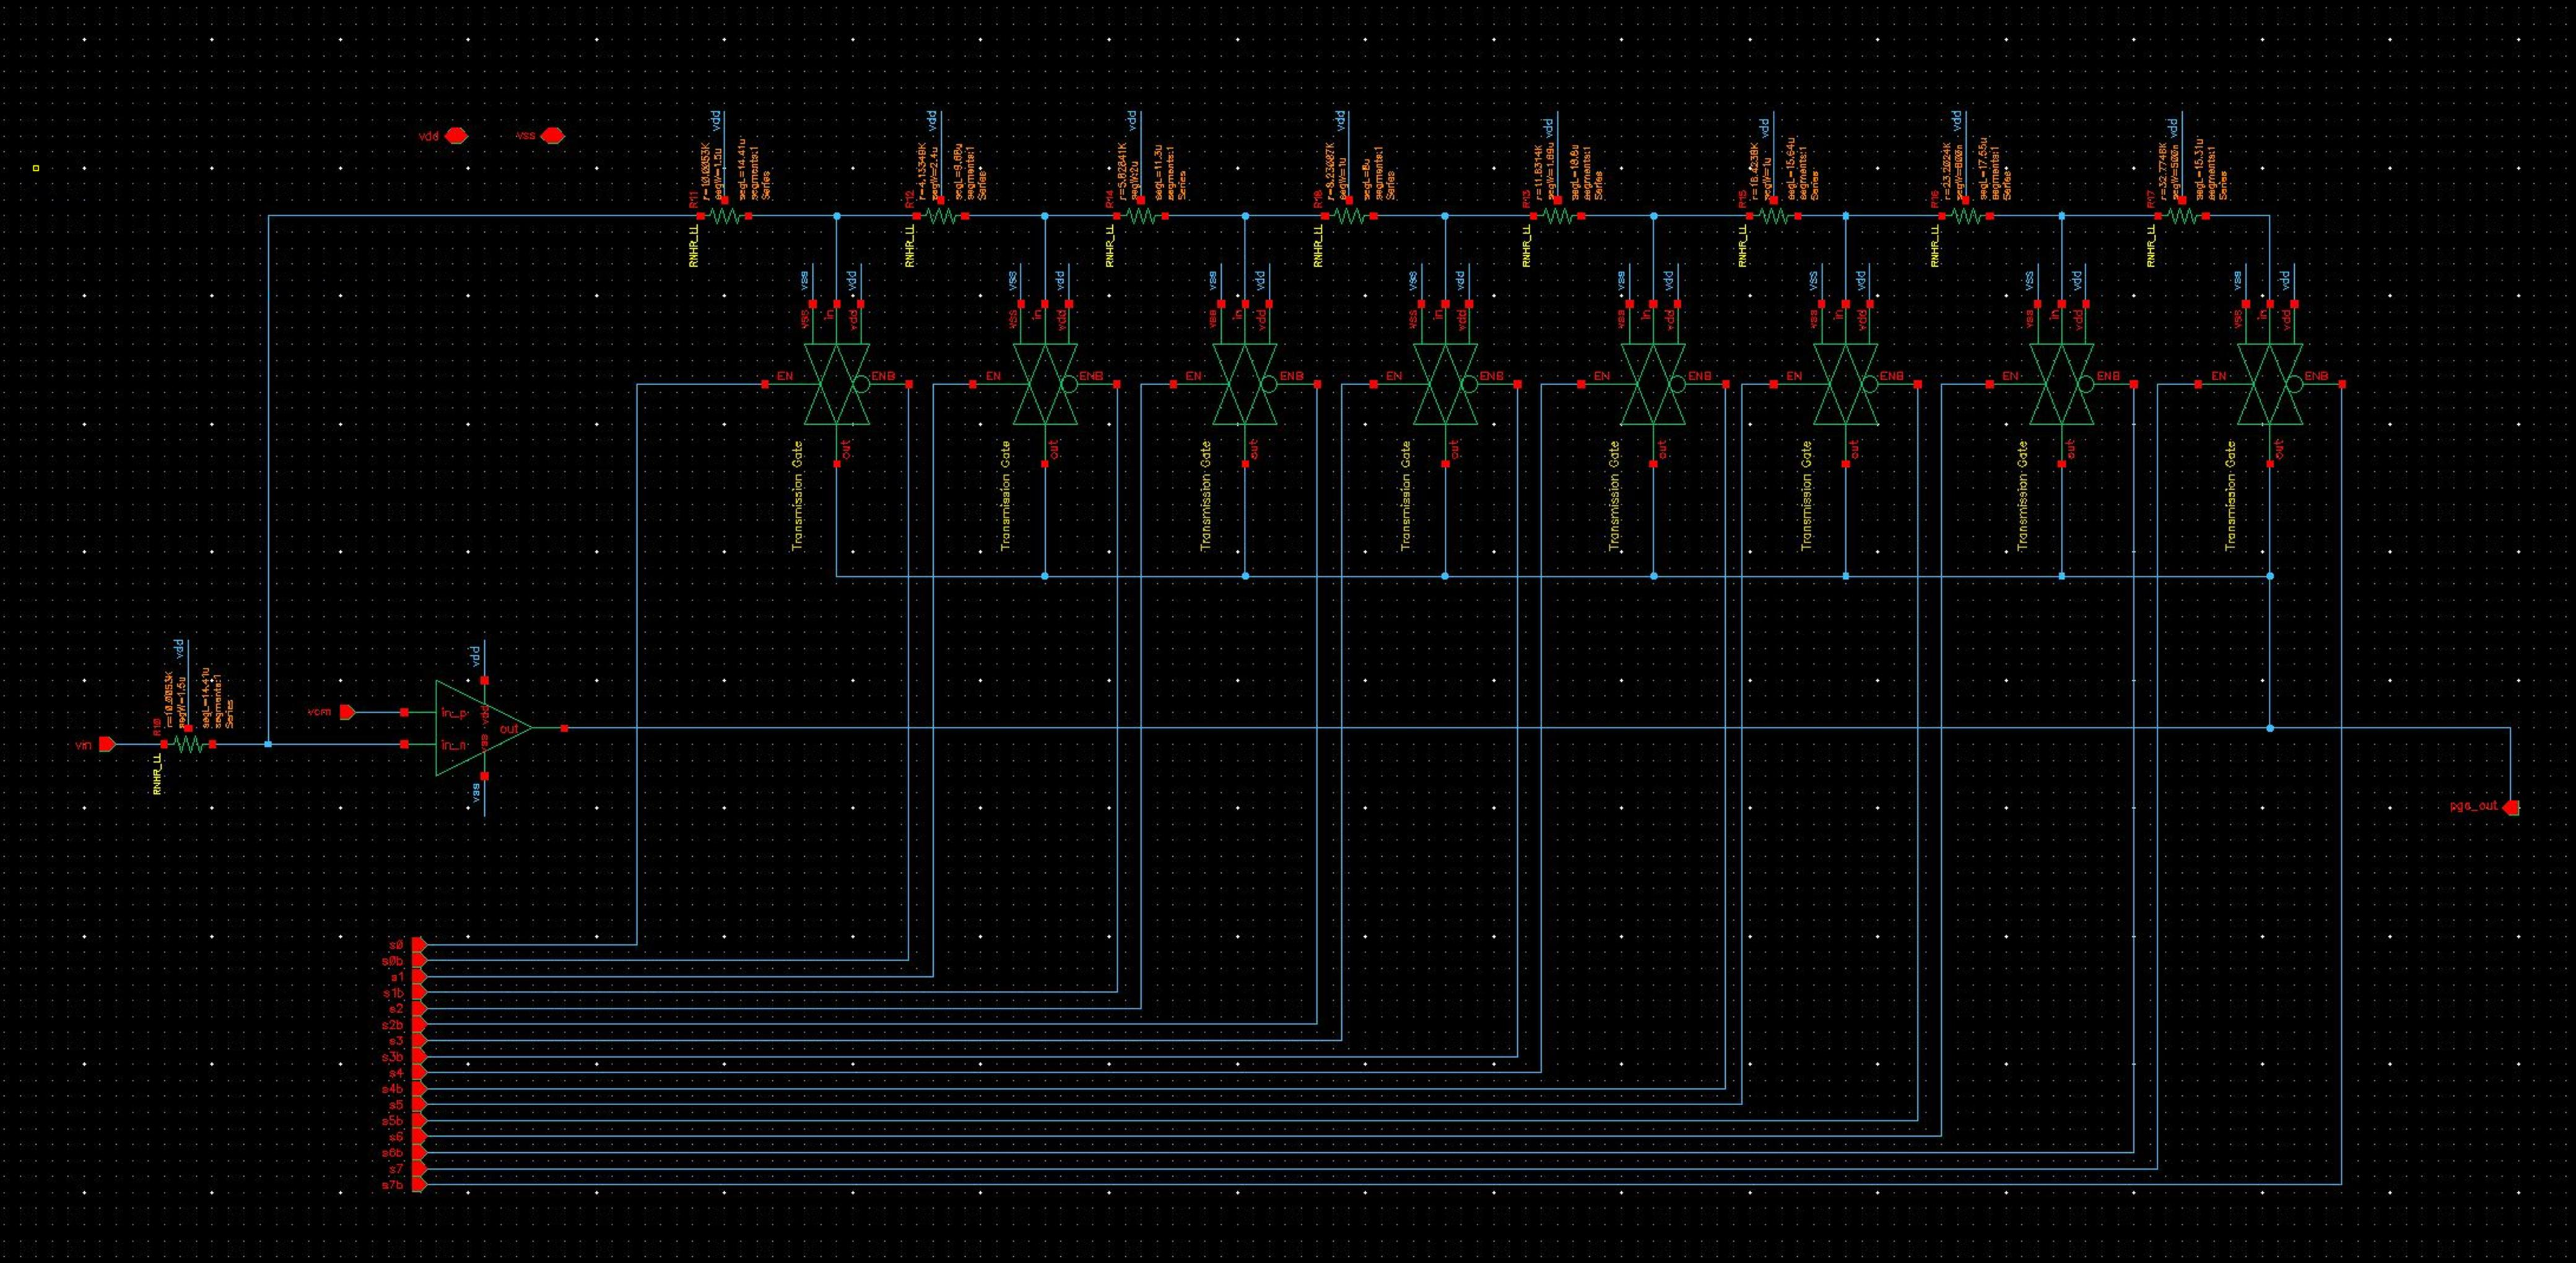
\includegraphics[width=0.96\textwidth]{figures/pga/pga_core.jpeg}

\medskip
\textbf{(b) Active low-pass filter}\par\smallskip
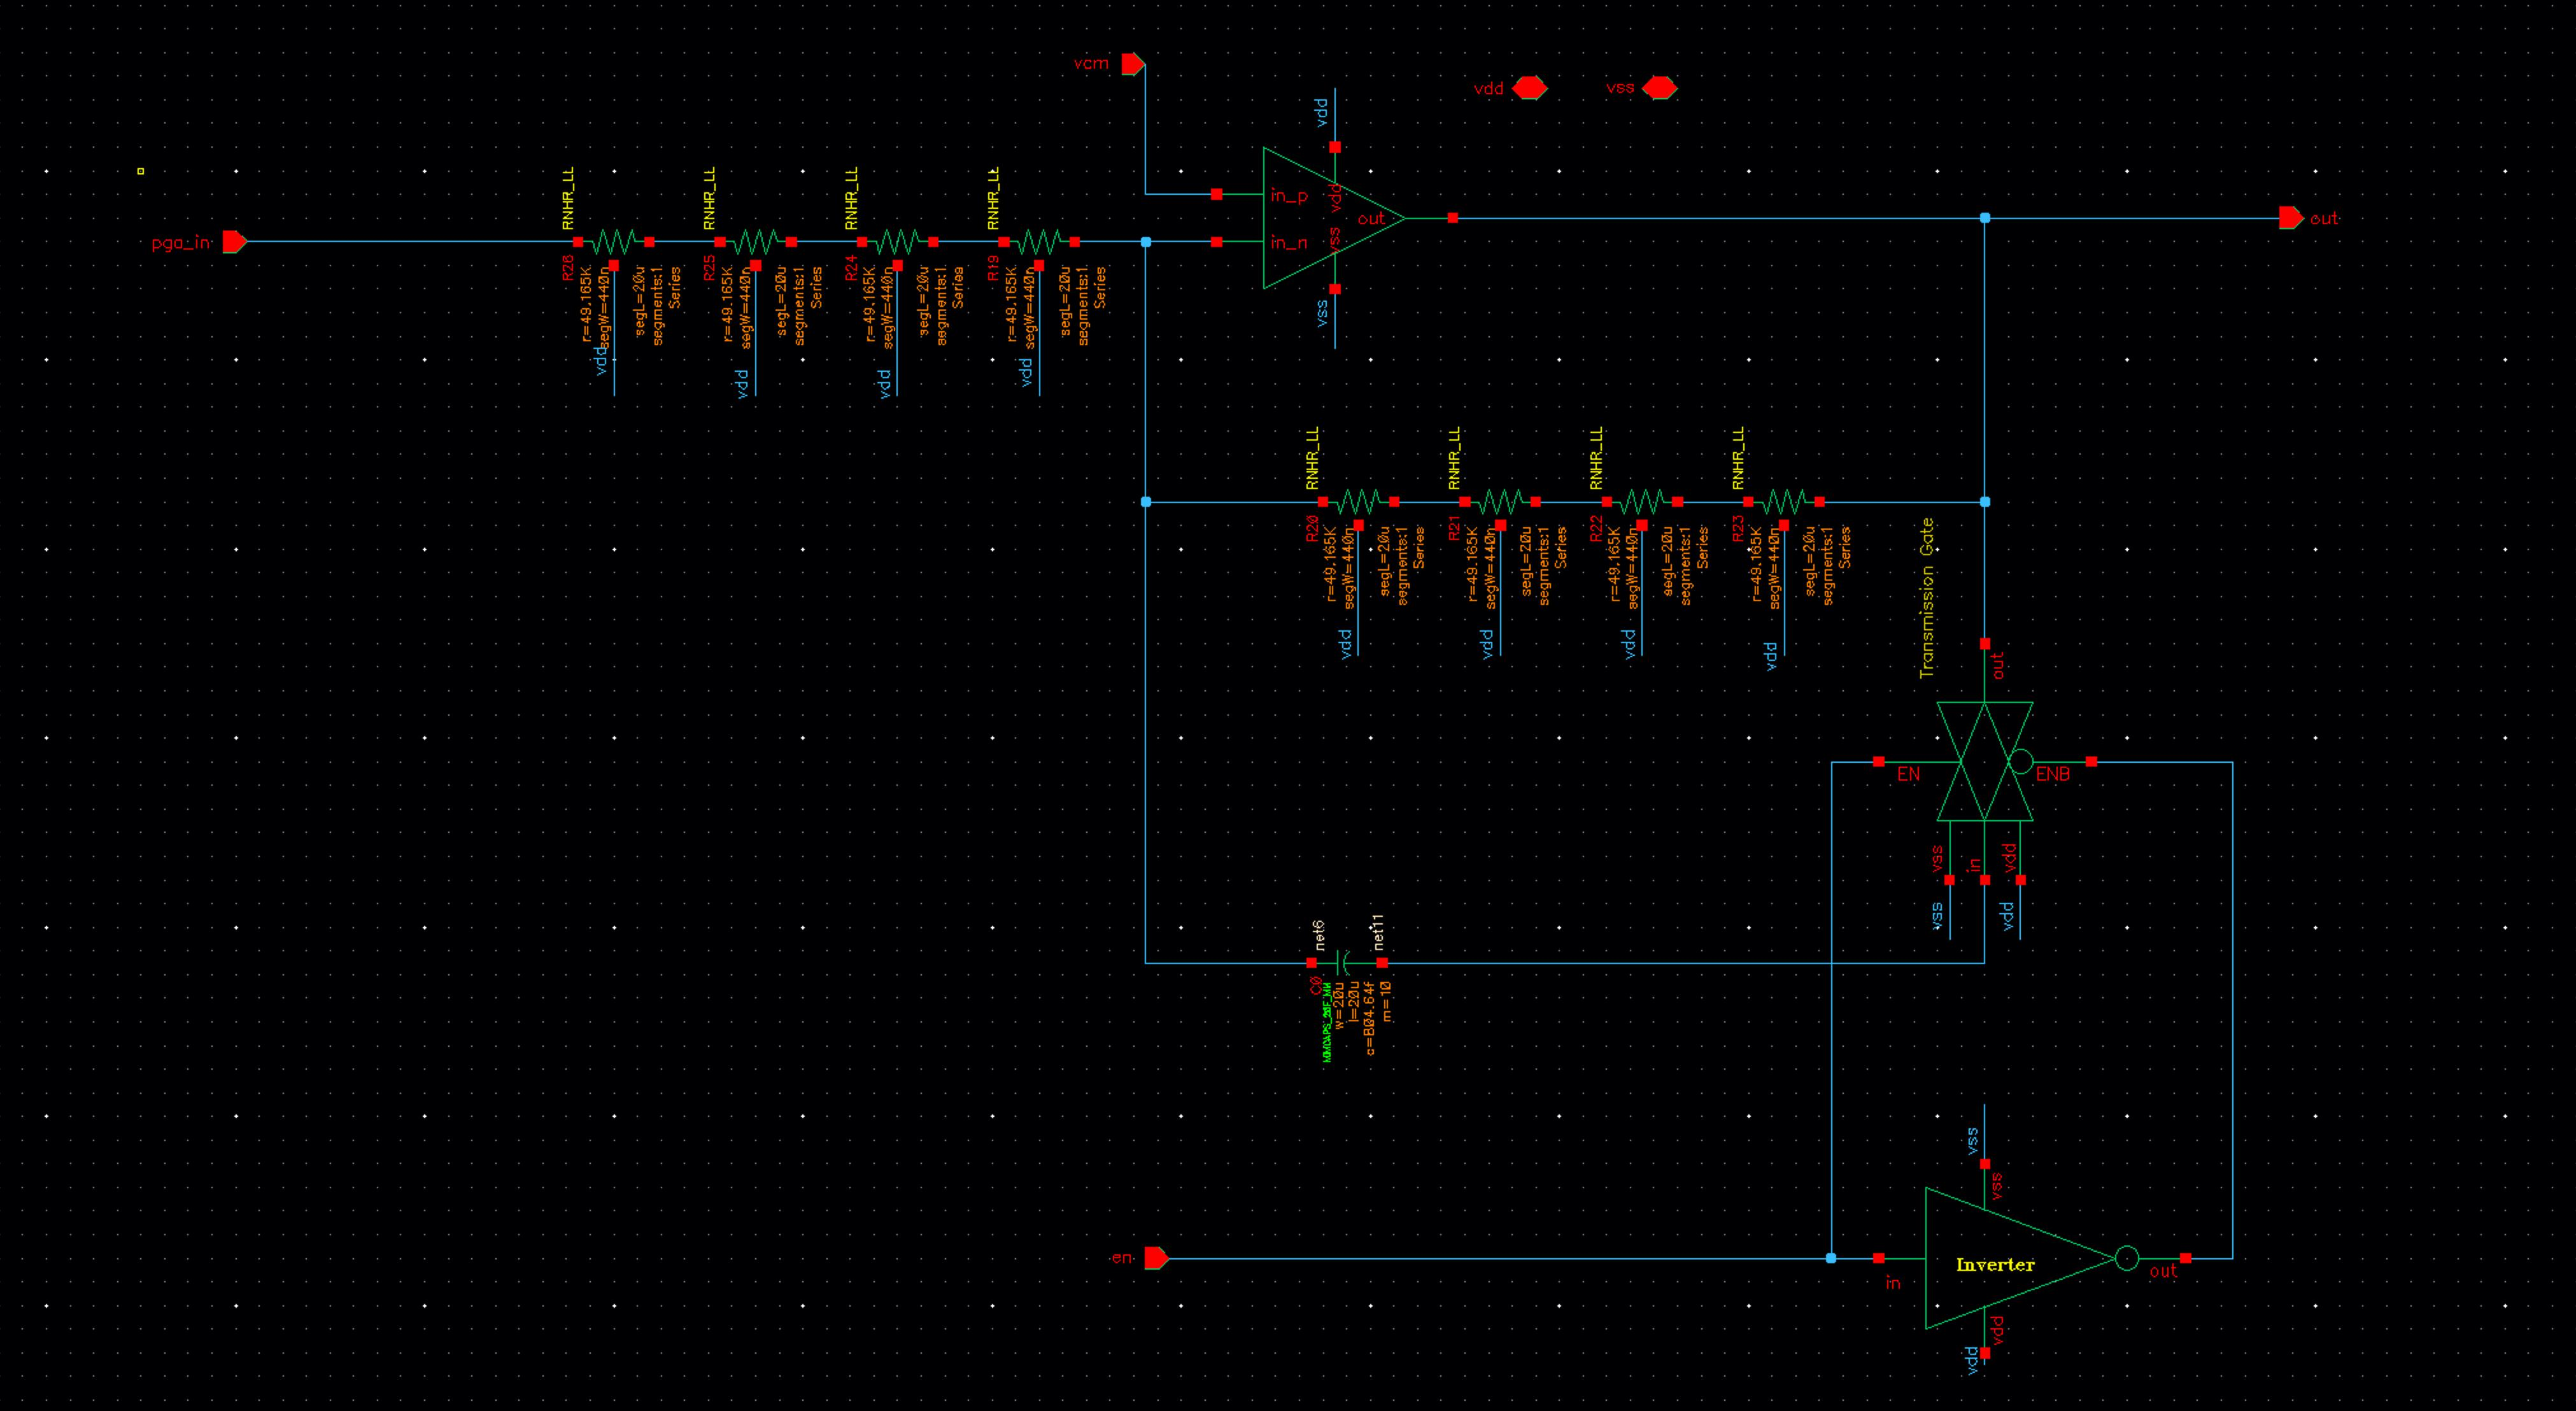
\includegraphics[width=0.90\textwidth]{figures/pga/lpf_schematic.jpeg}
\caption{Updated component schematics. The PGA core contains the programmable feedback network and its OPAMP; the LPF remains a separate enabled unity-gain stage.}
\label{fig:pga-component-schematics}
\end{figure}

The wrapper accepts \texttt{b0}--\texttt{b2}, \texttt{vin}, and \texttt{vcm}. The Controller generates eight one-hot outputs and their complements, and the wrapper routes them directly to the corresponding PGA-core switches. The PGA output remains available as \texttt{pga\_out}; the LPF is instantiated separately in the testbench so that the PGA and filter responses can still be measured independently.

\begin{figure}[p]
\centering
\textbf{(a) Controller and PGA wrapper}\par\smallskip
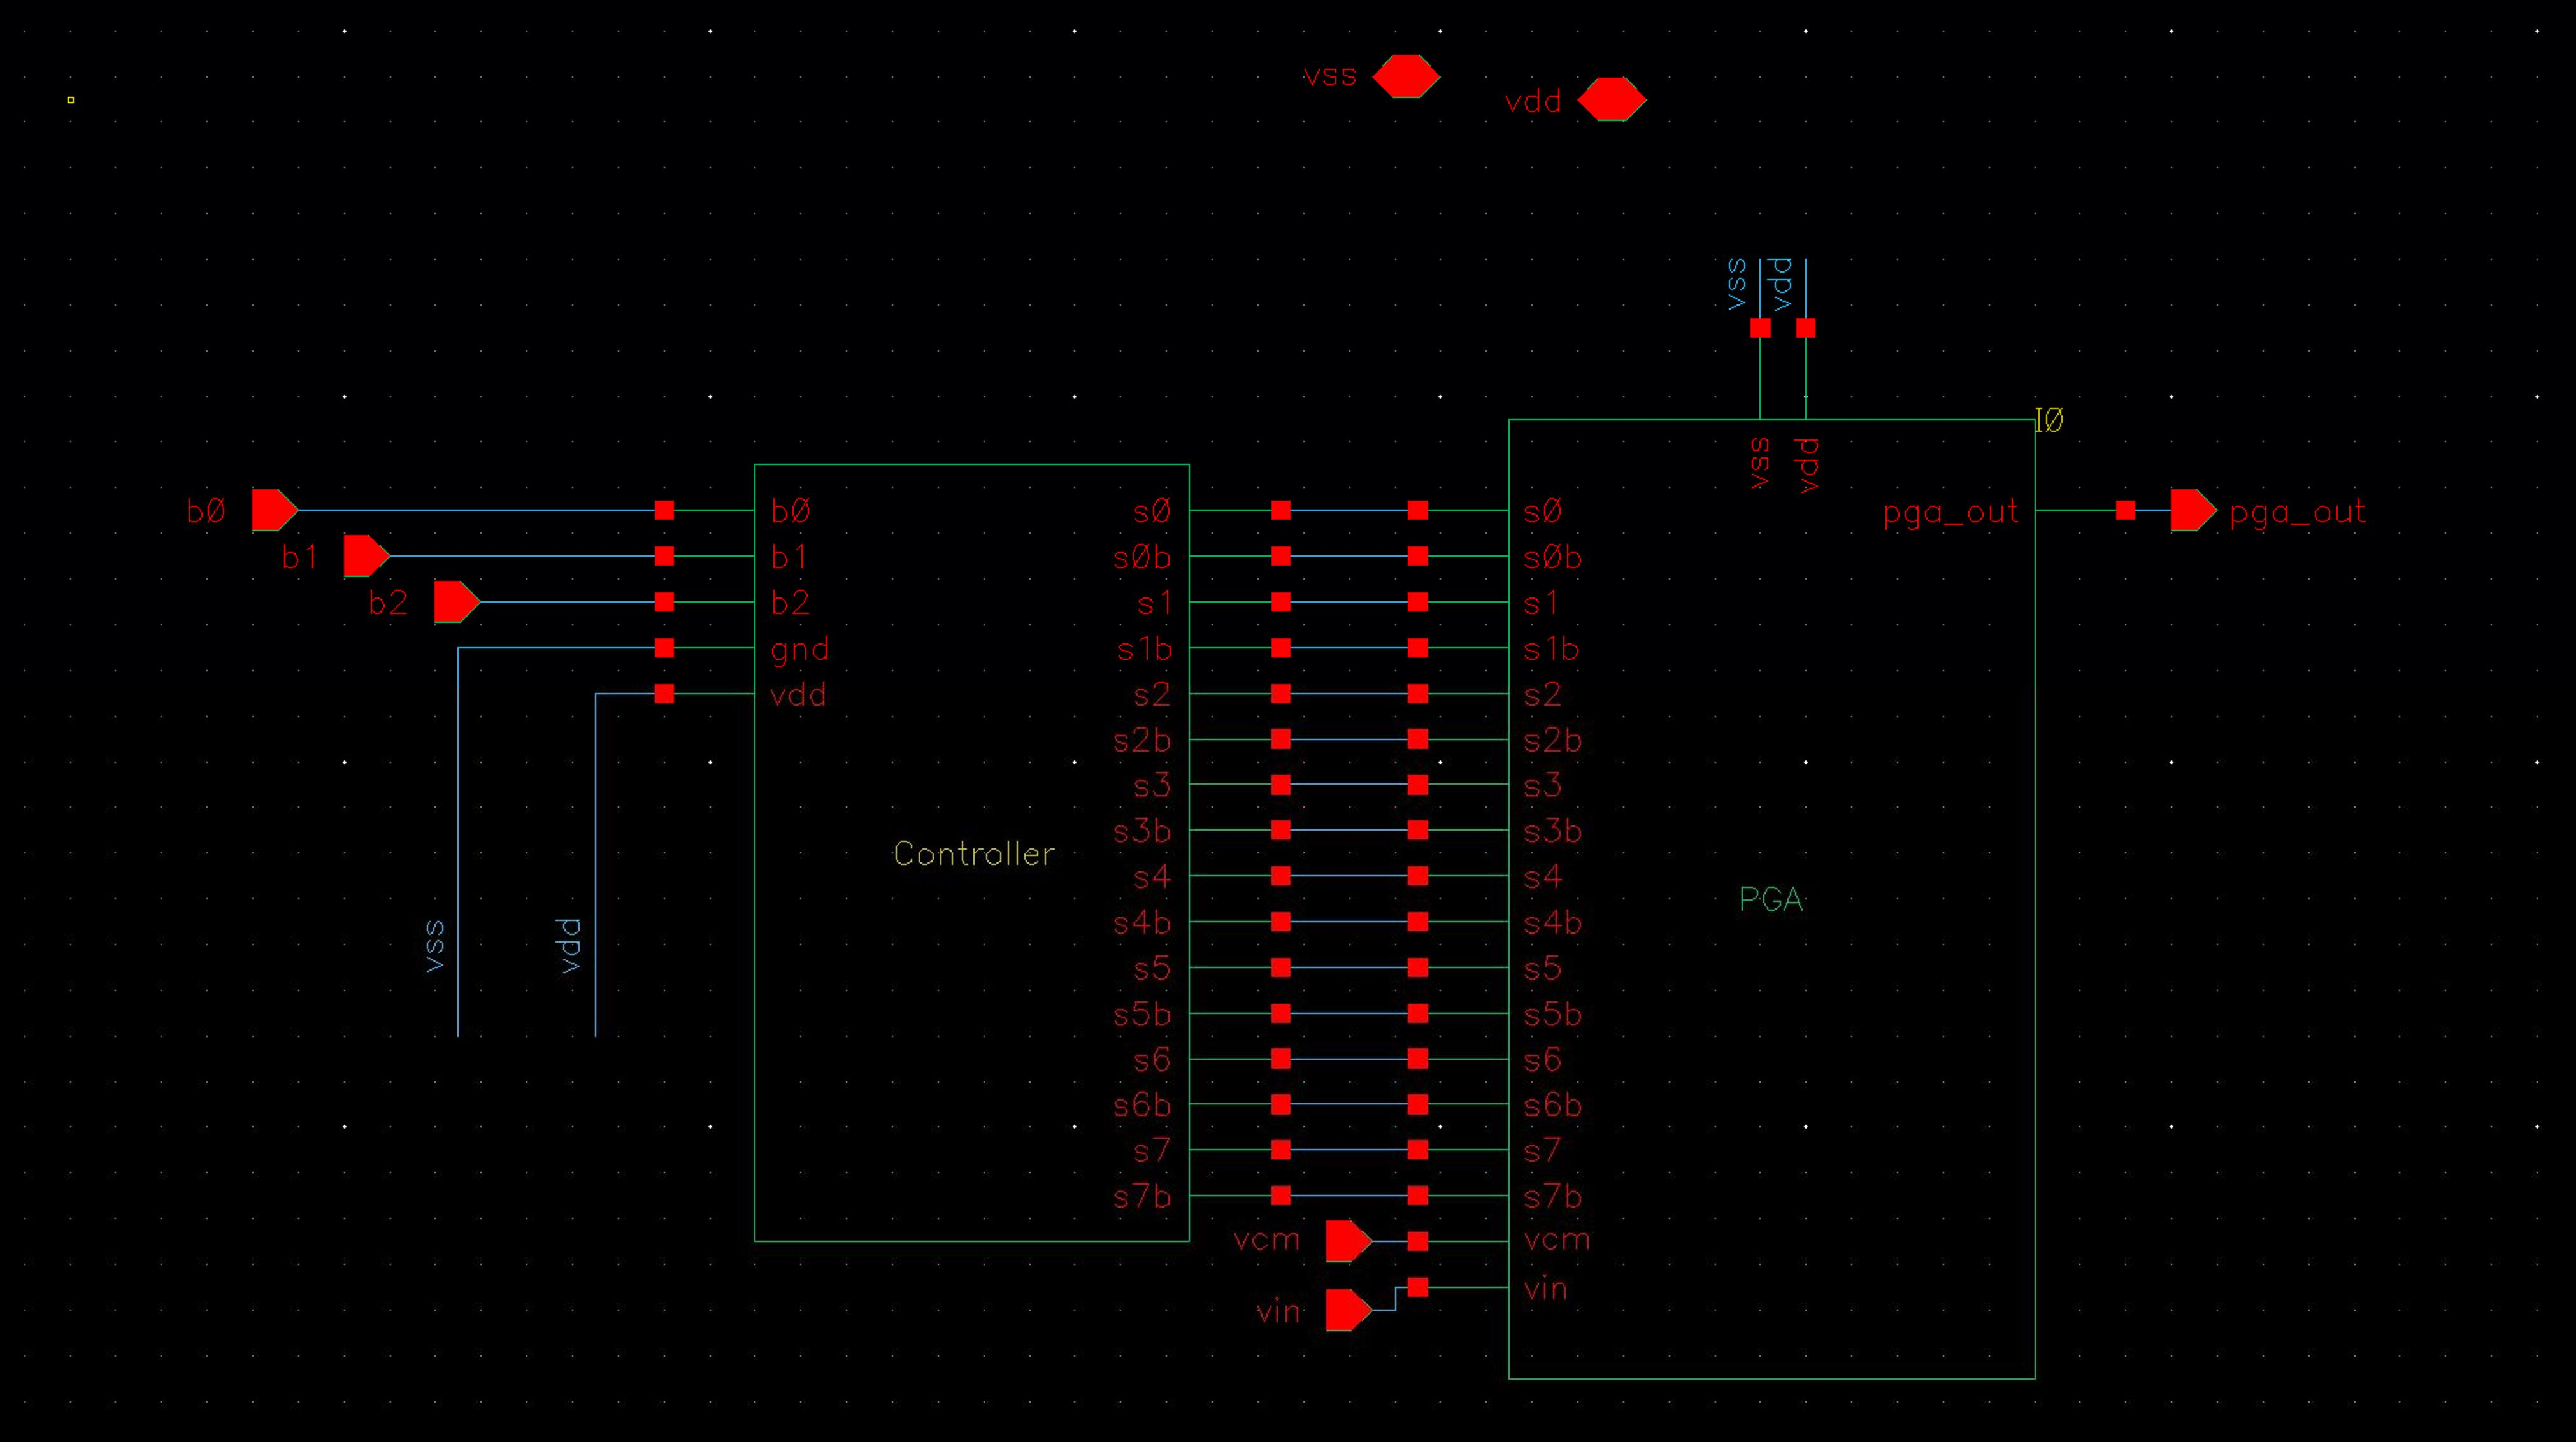
\includegraphics[width=0.72\textwidth]{figures/pga/pga_wrapper.jpeg}

\smallskip
\textbf{(b) Updated PGA and LPF testbench}\par\smallskip
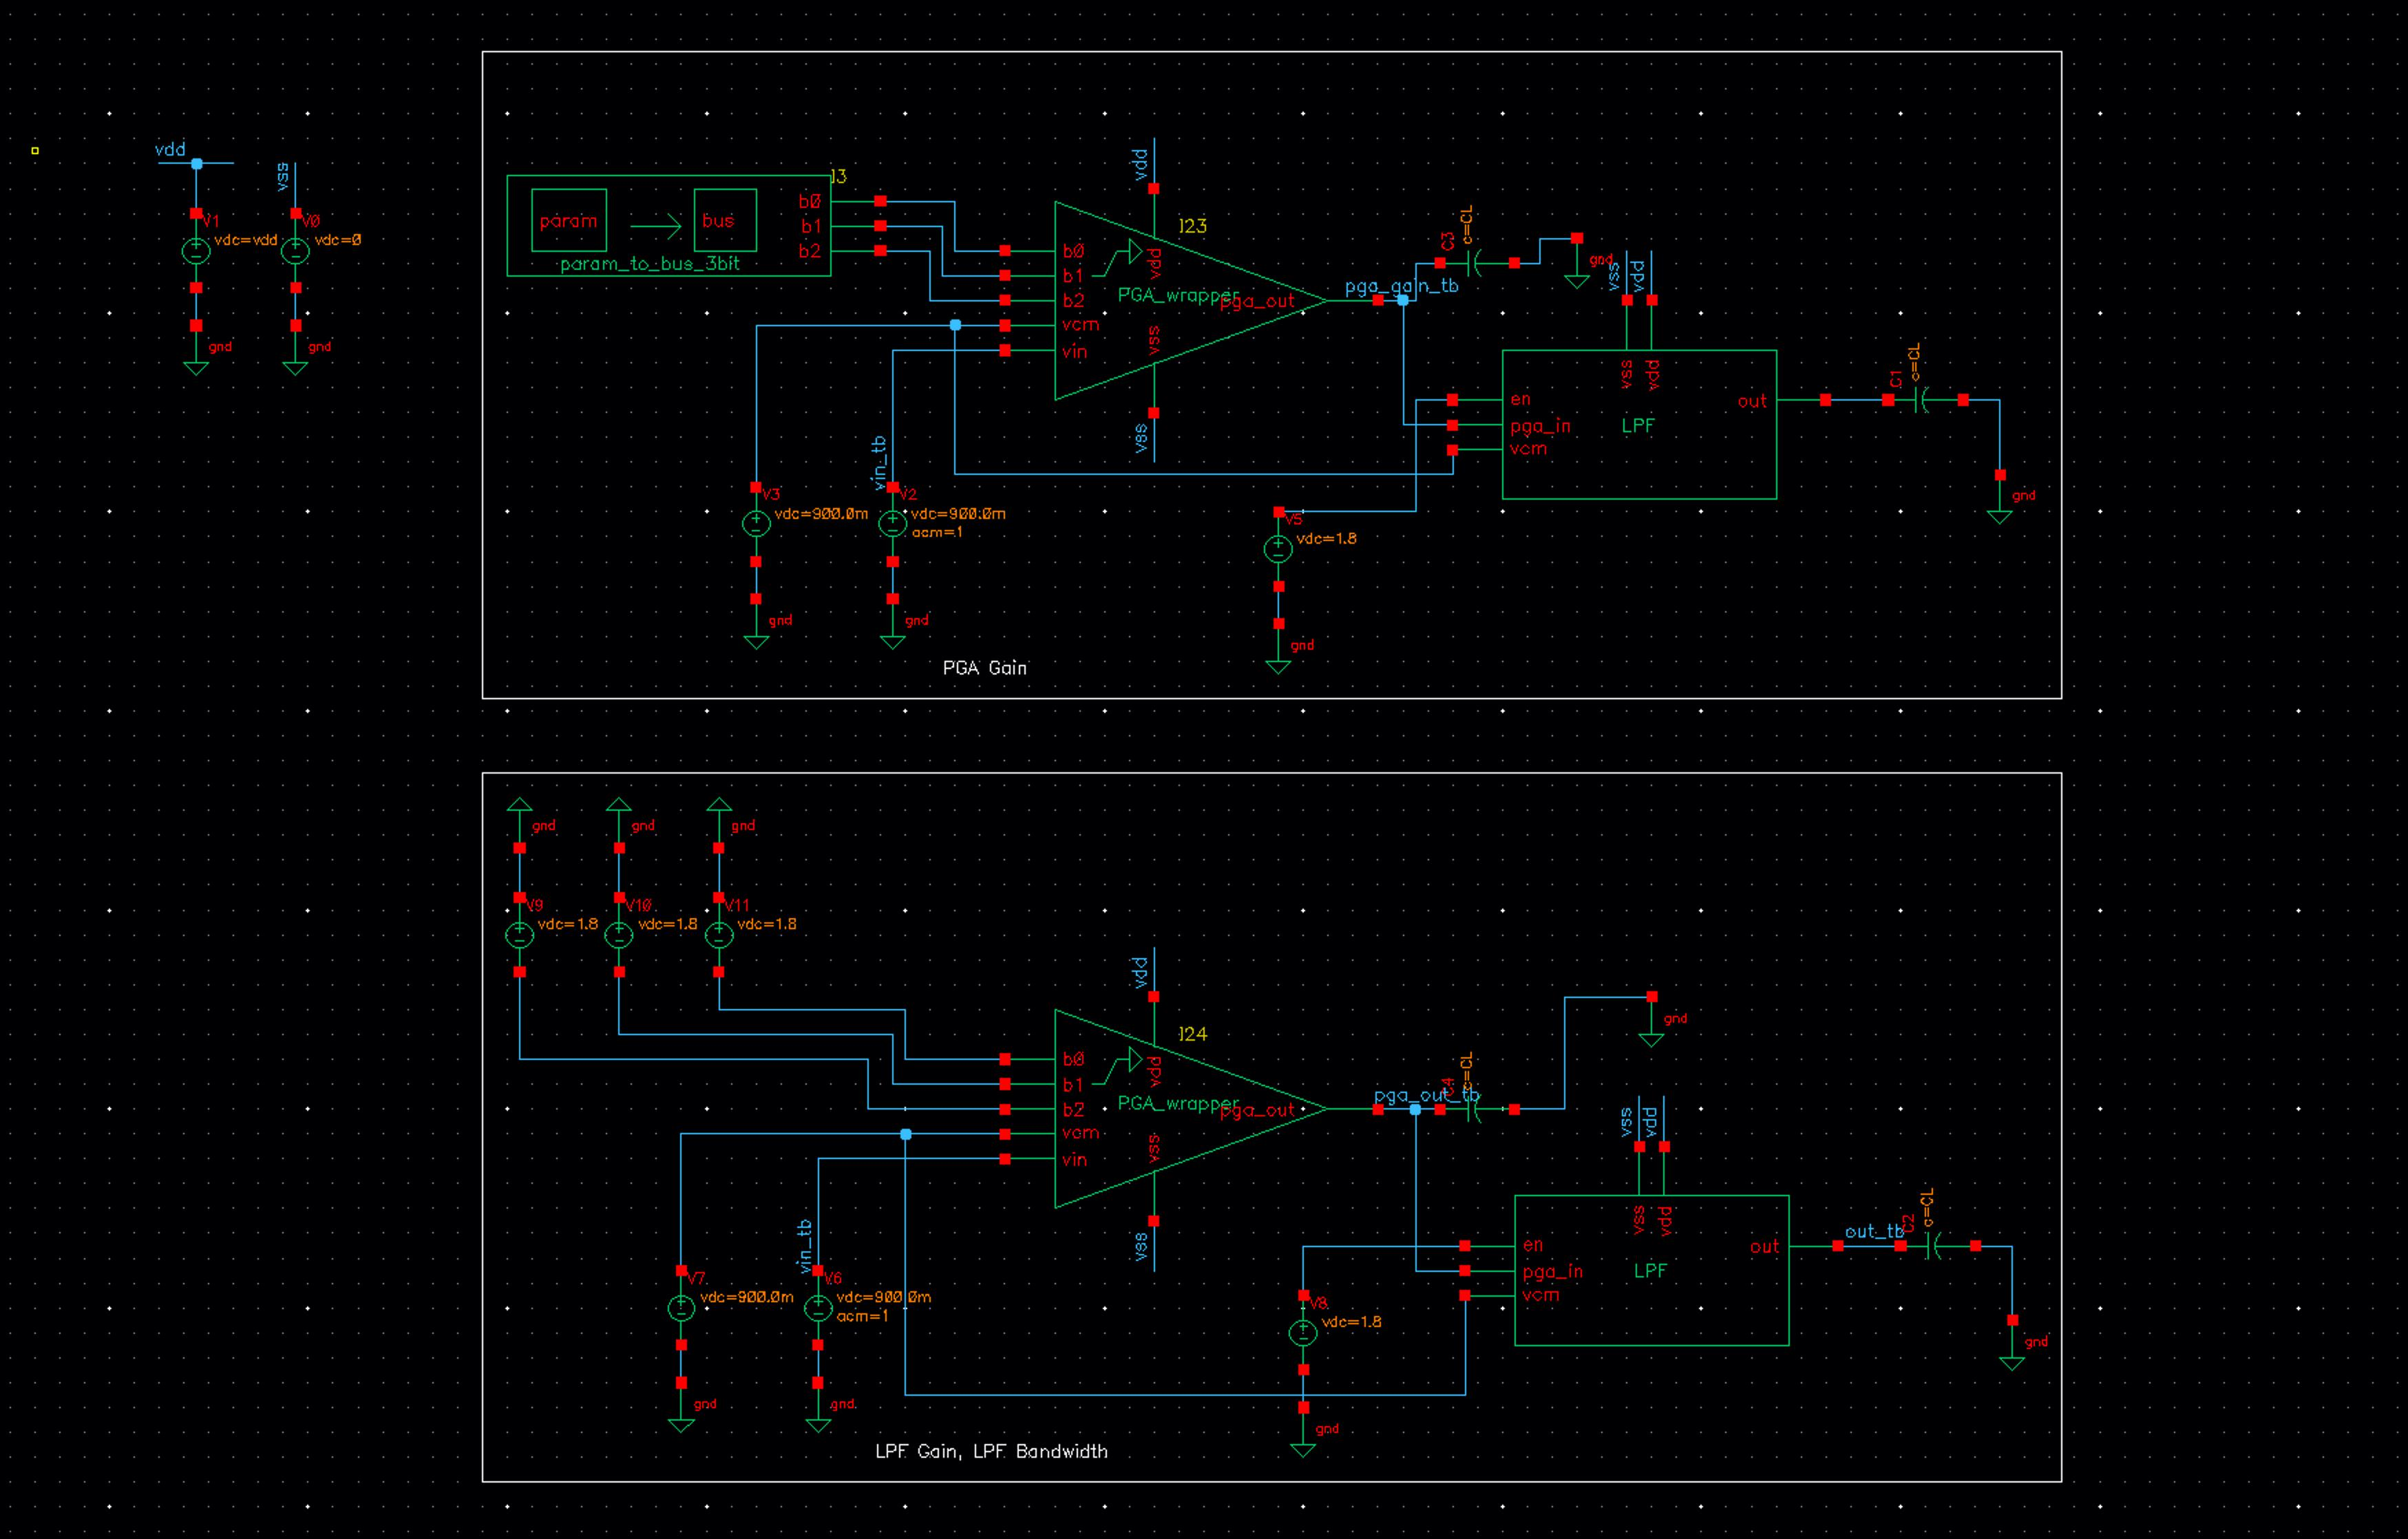
\includegraphics[width=0.88\textwidth]{figures/pga/pga_testbench_modular.jpeg}
\caption{Updated hierarchy and testbench. The upper test region drives the wrapper from a parameter-to-bus block for the gain-code sweep; the lower region uses explicit code sources for the LPF gain and bandwidth checks.}
\label{fig:pga-wrapper-testbench}
\end{figure}

These captures document the new hierarchy and wiring. No new ADE scalar, corner, or Monte Carlo export tied specifically to this refactoring was supplied, so the numerical tables in this chapter remain the verified schematic baseline.

\section{PGA feedback network and control}

For an ideal inverting stage referenced to \(\VCM\),
\begin{align}
\frac{V_{\mathrm{out}}-\VCM}{V_{\mathrm{in}}-\VCM}
&=-\frac{R_2}{R_1}, \\
G_{\mathrm{dB}}
&=20\log_{10}\!\left(\frac{R_2}{R_1}\right), \\
R_2
&=R_1\,10^{G_{\mathrm{dB}}/20}.
\end{align}
We set the target input resistance to \SI{10}{k\ohm}; the implemented RNHR value is approximately \SI{10.0051}{k\ohm}. Table~\ref{tab:pga-resistors} shows that the cumulative feedback string follows the eight 3 dB targets closely before switch and finite-loop effects.

\begin{table}[htbp]
\centering
\caption{Implemented cumulative PGA feedback values.}
\label{tab:pga-resistors}
\footnotesize
\begin{tabular}{@{}lrrr@{}}
\toprule
Code & Target (dB) & Cumulative $R_2$ (k$\Omega$) & Passive gain (dB) \\
\midrule
000 & 0  & 10.00530  & 0.00017 \\
001 & 3  & 14.13878  & 3.00381 \\
010 & 6  & 19.96719  & 6.00191 \\
011 & 9  & 28.19806  & 8.99996 \\
100 & 12 & 39.82946  & 11.99966 \\
101 & 15 & 56.25326  & 14.99853 \\
110 & 18 & 79.45566  & 17.99807 \\
111 & 21 & 112.23026 & 20.99777 \\
\bottomrule
\end{tabular}
\end{table}

Each feedback tap uses a CMOS transmission gate with a \texttt{P\_25\_LL} device of \SI{50}{\micro m}/\SI{240}{nm} and an \texttt{N\_25\_LL} device of \SI{25}{\micro m}/\SI{240}{nm}. With the switch in series with \SI{100}{k\ohm}, we swept the input from \SI{0.3}{V} to \SI{1.5}{V} and evaluated the switch resistance as
\begin{equation}
R_{\mathrm{sw}}(V)=\left|\frac{V_{\mathrm{in}}-V_{\mathrm{out}}}{I_{\mathrm{sw}}}\right|.
\end{equation}
The worst measured values are \(\Ron=\SI{232.1}{\ohm}\) and \(\Roff=\SI{38.81}{\giga\ohm}\). The finite \(\Ron\) is small relative to \SI{10}{k\ohm}, but its relative gain error is largest at code 000.

The behavioral Verilog-A controller decodes the three-bit input into eight one-hot signals and their complements, with \texttt{vth\_ratio=0.5}, \texttt{td=0}, and \texttt{tr=tf=1 ns}. Sweeping all eight gain codes through the complete PGA testbench verifies the static decode path together with the MUX and feedback network.

% TODO(figure readability): Replace the transmission-gate screenshot with a larger resistance crop if available. The exact worst-case values are reported in the text because the on-resistance is compressed by the linear GOhm-scale axis.
\begin{figure}[htbp]
\centering
\begin{minipage}[t]{0.47\textwidth}
\centering
\textbf{(a) Nominal gain versus code}\par\smallskip
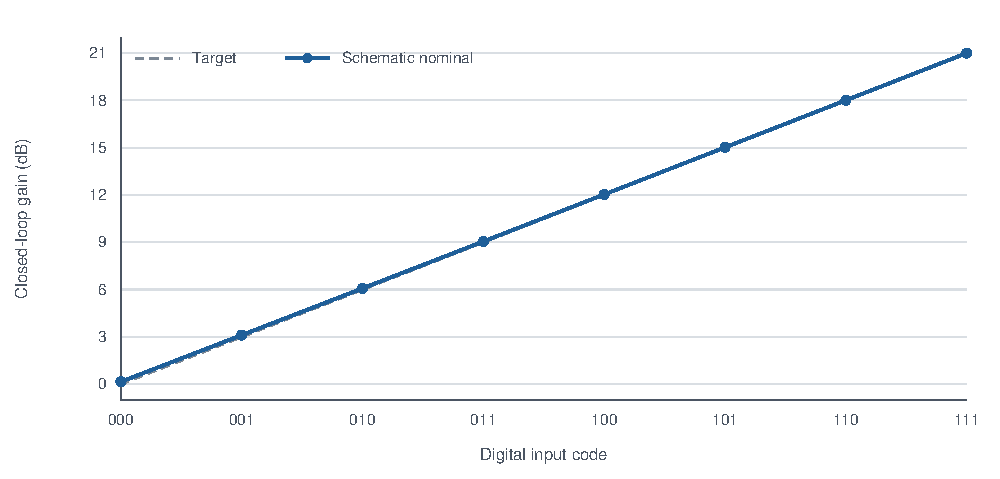
\includegraphics[width=\linewidth]{figures/pga/gain_vs_code.pdf}
\end{minipage}\hfill
\begin{minipage}[t]{0.47\textwidth}
\centering
\textbf{(b) TG on/off resistance}\par\smallskip
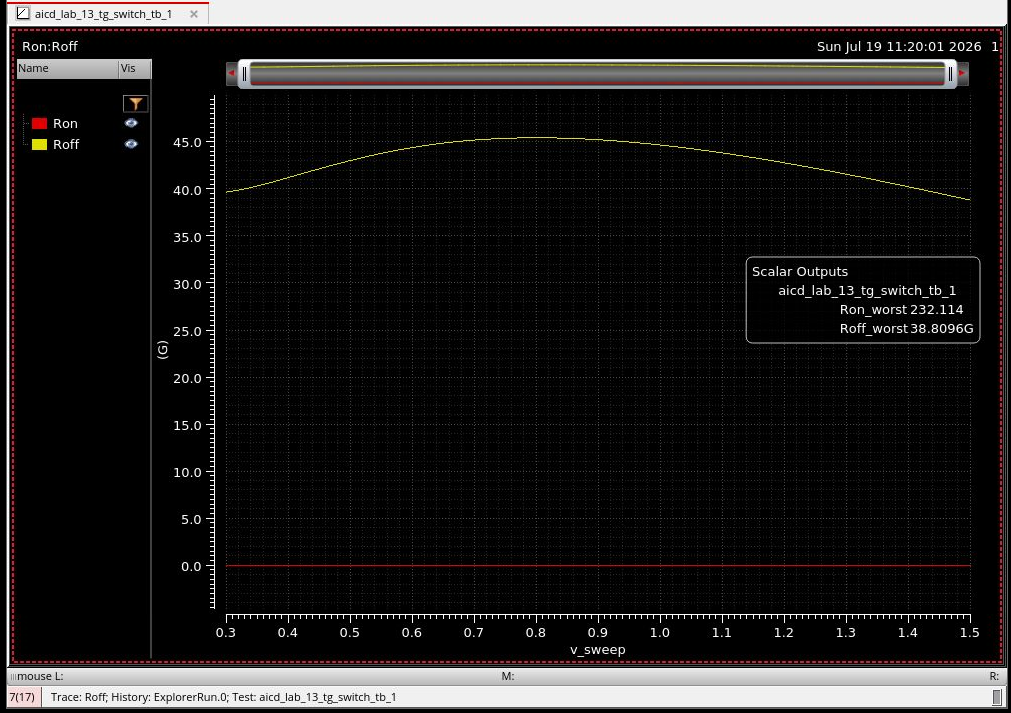
\includegraphics[width=\linewidth]{figures/pga/tg_resistance.png}
\end{minipage}
\caption{Nominal PGA gain versus digital code and transmission-gate resistance over the \SIrange{0.3}{1.5}{V} input sweep. Exact resistance limits are reported in the text.}
\label{fig:pga-gain-tg}
\end{figure}

\section{Active low-pass filter}

The second inverting stage uses equal input and feedback resistance. Each path contains four series RNHR elements of approximately \SI{401.65}{k\ohm}, giving approximately \SI{1.6066}{M\ohm} per path. The \SI{884.64}{fF} feedback capacitor is connected through an enable transmission gate.

Ignoring the enable-switch resistance and finite OPAMP response, the transfer function and pole are
\begin{align}
H(j\omega)
&=-\frac{R_2/R_1}{1+j\omega R_2 C}, \\
f_{\mathrm{p,ideal}}
&=\frac{1}{2\pi R_2 C}
\approx\SI{111.98}{kHz}.
\end{align}
The large resistance lets us reach the target time constant with the implemented \SI{884.64}{fF} capacitor. Reducing the total below the course guideline of approximately \SI{1}{M\ohm} would require a larger capacitor and a coordinated redesign of the filter, layout, and simulations. We therefore retained the \SI{1.6066}{M\ohm} value and treat it as an area and layout risk. The enable-switch resistance and finite OPAMP response shift the simulated -3 dB bandwidth to \SI{100.1}{kHz}, approximately \SI{10.6}{\percent} below the first-order estimate and within the allowed \SIrange{50}{150}{kHz} range.

% TODO(figure readability): Replace the LPF magnitude and phase panels with larger native exports if available. The curves are readable at the current scale, but the exact -3 dB value should be taken from the scalar result rather than the screenshot.
\begin{figure}[htbp]
\centering
\begin{minipage}[t]{0.48\textwidth}
\centering
\textbf{(a) Magnitude and -3 dB crossing}\par\smallskip
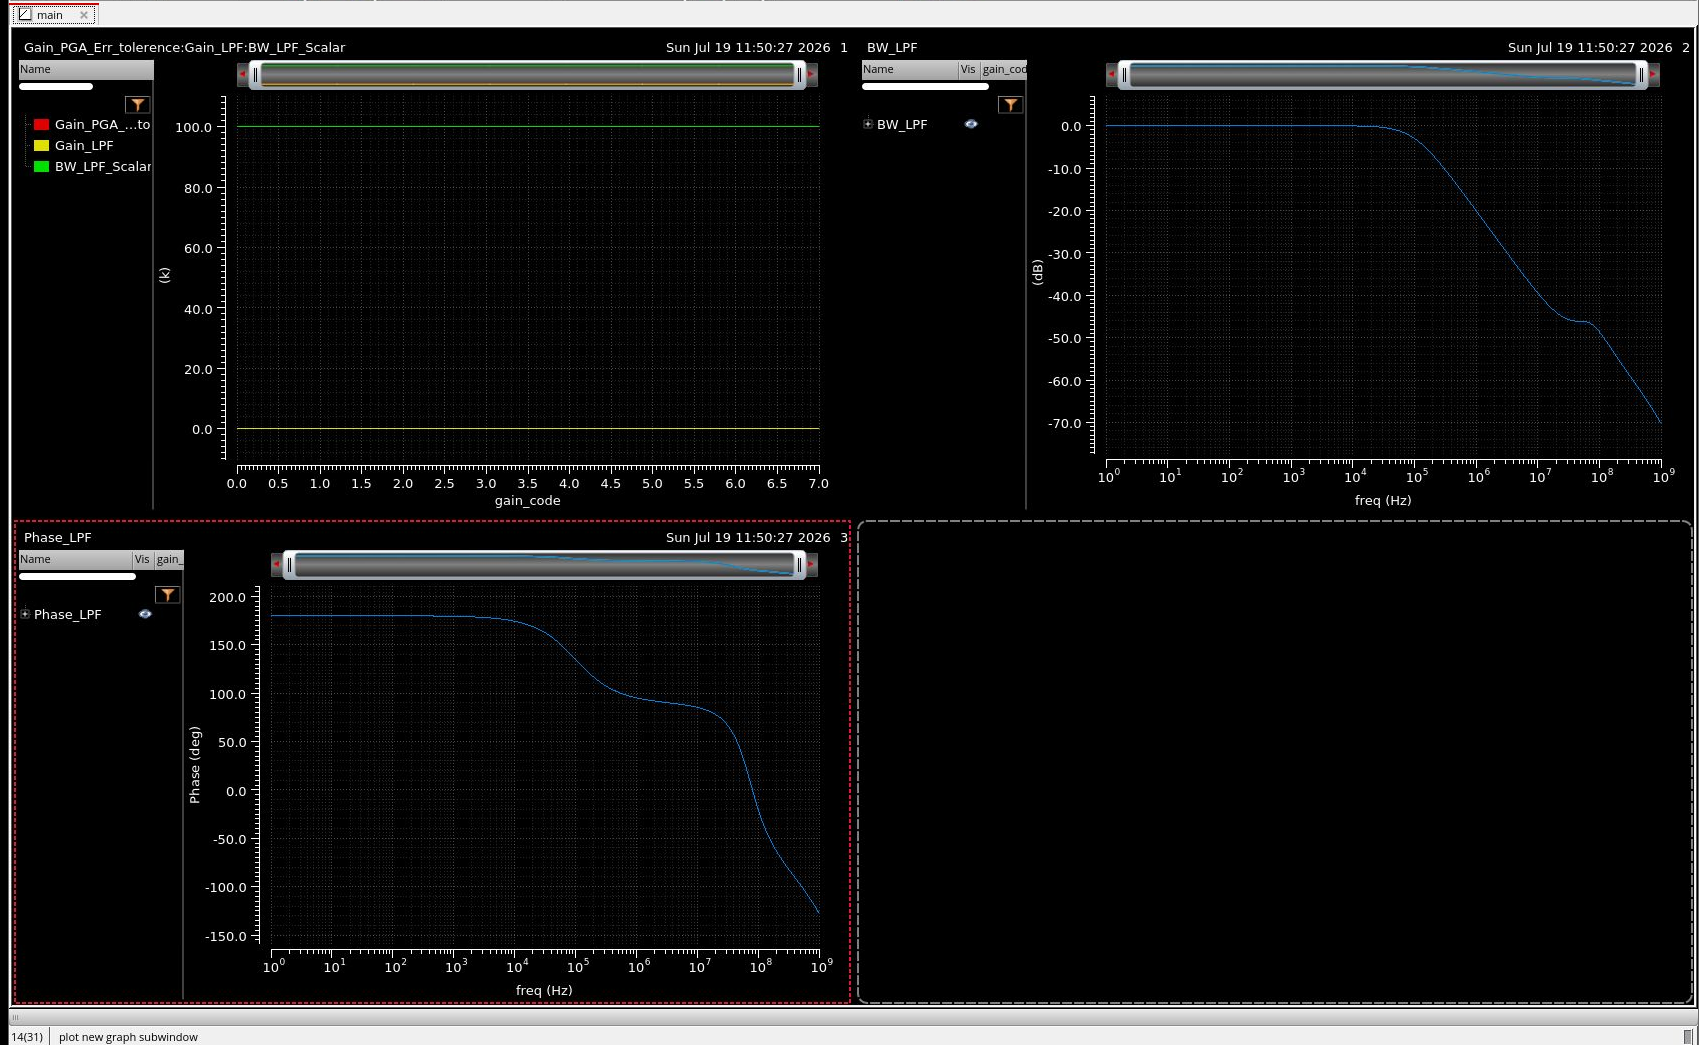
\includegraphics[width=\linewidth,trim=850 523 0 0,clip]{figures/pga/lpf_response.png}
\end{minipage}\hfill
\begin{minipage}[t]{0.48\textwidth}
\centering
\textbf{(b) Phase}\par\smallskip
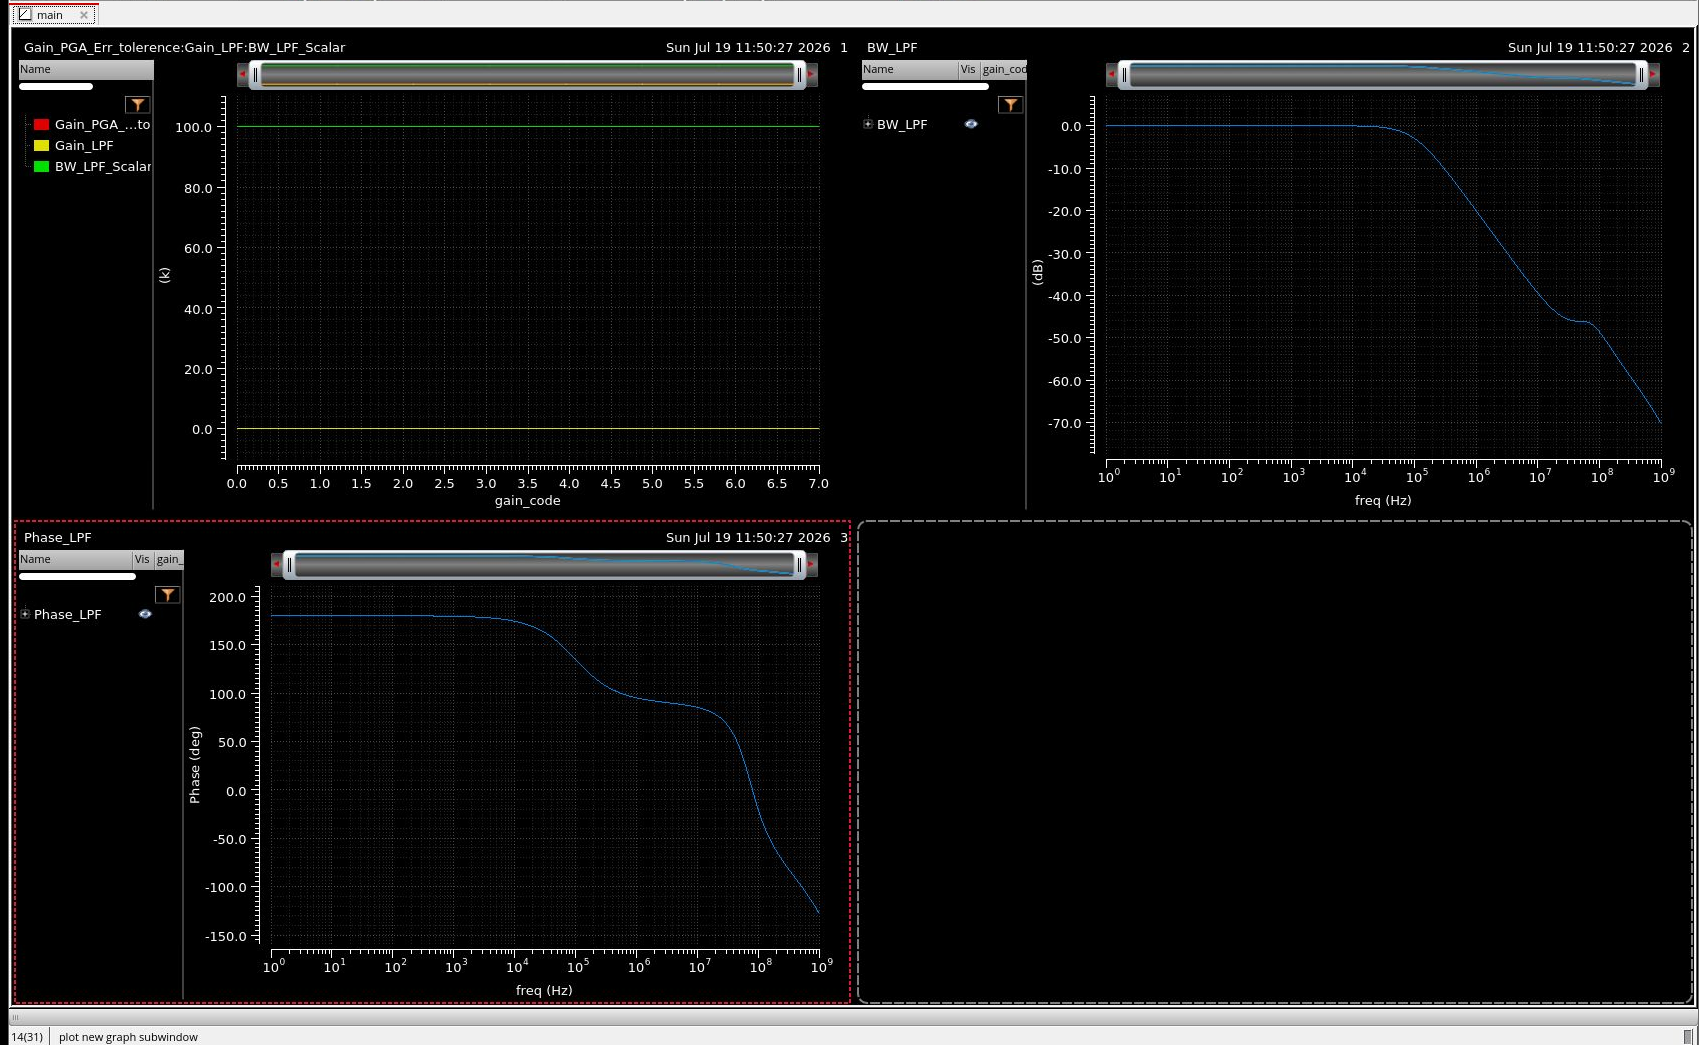
\includegraphics[width=\linewidth,trim=0 0 849 522,clip]{figures/pga/lpf_response.png}
\end{minipage}
\caption{Nominal LPF magnitude and phase response. The low-frequency phase near \SI{180}{\degree} is consistent with an inverting stage; the scalar -3 dB bandwidth is \SI{100.1}{kHz}.}
\label{fig:lpf-response}
\end{figure}

\section{Nominal, corner, and Monte Carlo results}

% LAYOUT HANDOFF: Add post-layout data to Tables 7(a) and 7(b) in the form
% PEX (schematic). Use the same eight codes, 64-corner grid, and 100 Monte
% Carlo points per code. Keep all schematic values unchanged. The LPF PEX
% comparison belongs in chapters/layout.tex and should not be repeated here.

The nominal sweep covers \texttt{gain\_code=0:1:7} from \SI{1}{Hz} to \SI{1}{GHz} with 80 logarithmic points per decade. PGA gain is evaluated at \SI{1}{kHz} relative to the target $3\,\texttt{gain\_code}$. All eight nominal gains satisfy the $\pm\SI{1.5}{dB}$ window. An independent rerun changes the reported errors by no more than \SI{0.0142}{dB} and does not change the pass status.

Across 64 PVT corners, every PGA code and both LPF scalar checks pass. The largest PGA excursion is \SI{1.221}{dB} at code 000, leaving \SI{0.279}{dB} to the upper limit. The LPF bandwidth spans \SIrange{72.88}{121.8}{kHz}.

\begin{table}[H]
\centering
\caption{Course Table~7(a), schematic values for codes 000--011.}
\label{tab:pga-table7-low}
\scriptsize
\renewcommand{\arraystretch}{0.92}
\begin{tabularx}{\textwidth}{@{}Yrrrr@{}}
\toprule
Parameter & 000 (dB) & 001 (dB) & 010 (dB) & 011 (dB) \\
\midrule
Target / corner tolerance & $0\pm1.5$ & $3\pm1.5$ & $6\pm1.5$ & $9\pm1.5$ \\
Typical & 0.1463 & 3.1058 & 6.0723 & 9.0475 \\
Corner minimum & 0.0500 & 3.0319 & 6.0165 & 9.0117 \\
Corner maximum & 1.2210 & 3.8869 & 6.6357 & 9.4463 \\
Passed / total corners & 64/64 & 64/64 & 64/64 & 64/64 \\
\midrule
MC minimum & 0.0793 & 3.0511 & 6.0249 & 8.9976 \\
MC maximum & 0.2248 & 3.1748 & 6.1417 & 9.1179 \\
MC mean & 0.1461 & 3.1059 & 6.0721 & 9.0474 \\
MC standard deviation & 0.02701 & 0.02387 & 0.02253 & 0.02347 \\
MC yield & 100/100 & 100/100 & 100/100 & 100/100 \\
\bottomrule
\end{tabularx}
\end{table}

\begin{table}[H]
\centering
\caption{Course Table~7(b), schematic values for codes 100--111.}
\label{tab:pga-table7-high}
\scriptsize
\renewcommand{\arraystretch}{0.92}
\begin{tabularx}{\textwidth}{@{}Yrrrr@{}}
\toprule
Parameter & 100 (dB) & 101 (dB) & 110 (dB) & 111 (dB) \\
\midrule
Target / corner tolerance & $12\pm1.5$ & $15\pm1.5$ & $18\pm1.5$ & $21\pm1.5$ \\
Typical & 12.0304 & 15.0165 & 18.0059 & 20.9967 \\
Corner minimum & 12.0049 & 14.9998 & 17.9823 & 20.9546 \\
Corner maximum & 12.3129 & 15.2094 & 18.1299 & 21.0980 \\
Passed / total corners & 64/64 & 64/64 & 64/64 & 64/64 \\
\midrule
MC minimum & 11.9758 & 14.9724 & 17.9524 & 20.9303 \\
MC maximum & 12.0878 & 15.0652 & 18.0525 & 21.0686 \\
MC mean & 12.0292 & 15.0152 & 18.0055 & 20.9966 \\
MC standard deviation & 0.02074 & 0.02022 & 0.02069 & 0.02288 \\
MC yield & 100/100 & 100/100 & 100/100 & 100/100 \\
\bottomrule
\end{tabularx}
\end{table}

The Monte Carlo analysis uses variation \texttt{All}, 100 points per code, standard random sampling, seed 12345, and first point 1. All PGA and LPF outputs pass 100/100 points. PGA standard deviation is \SIrange{0.02022}{0.02701}{dB}. LPF bandwidth is \SIrange{82.8}{119.5}{kHz}, with a \SI{100.0}{kHz} mean and \SI{6.796}{kHz} standard deviation.

The archive contains no full all-code PGA AC magnitude/phase export or measured \texttt{010} to \texttt{101} switching waveform. The static sweeps support the tabulated gains; dynamic switching remains unverified.
